% Fragmento para incorporação ao relatório principal do projeto PRO3474.
% Pacotes pressupostos no preâmbulo do documento que incorporar este arquivo:
%   inputenc (utf8), fontenc (T1), graphicx, pdflscape (já exigido pela matriz de NDD).
% Figuras referenciadas em figures/ (caminho relativo a este arquivo), em PDF vetorial.
% Versões PNG (300 dpi) das mesmas figuras acompanham os arquivos, caso o relatório
% seja compilado sem suporte a PDF em \includegraphics.
% Referências cruzadas externas usadas: fig:confianca_geral e sec:clusters (Análise dos clientes).

\section{MODELAGEM FUNCIONAL (ENTREGA 2)}
\label{sec:modelagem_funcional}

Seguindo \citeonline{rozenfeld2006gestao}, a equipe descreveu o produto por suas funções, sem referência a princípios físicos, para que a hipótese de solução em estudo não restringisse a busca de alternativas nas etapas seguintes. Cada função recebeu a forma de um par verbo + substantivo. O modelo tem duas partes: a função total e o seu desdobramento em uma estrutura de funções ligadas por fluxos de energia, material e sinal.

A equipe modelou o sistema completo, incluindo as trocas de informação com sistemas que a Riachuelo já opera: meio de pagamento, caixa, controle de estoque e antifurto da saída da loja. Esses sistemas ficaram fora da fronteira e aparecem no modelo como origem ou destino de sinais. A predominância de fluxos de sinal exigiu a principal adaptação do método, já que os exemplos do método tratam de produtos com predomínio de fluxos de material e energia, como a lavadora de roupas.

\subsection{Função total e fronteira do sistema}
\label{sec:funcao_total}

Para chegar à função total, a equipe seguiu o roteiro de Gomes Ferreira reproduzido por \citeonline{rozenfeld2006gestao}, partindo das entradas e saídas do sistema: classificou-as por tipo de fluxo, estabeleceu o estado de cada uma, destacou os fluxos principais e expressou a transformação entre eles por um par verbo + substantivo. Dois fluxos principais atravessam o sistema. O de material leva a peça do estado livre ao estado liberado. O de sinal reúne a seleção da peça e a confirmação de pagamento em um vínculo entre ambas. A função total, \emph{conciliar peça e pagamento}, nomeia o ponto em que os dois fluxos se encontram: a peça só muda de estado quando o pagamento correspondente é confirmado (Figura~\ref{fig:funcao_total}).

\begin{figure}[htbp]
    \centering
    \caption{Diagrama de caixa preta do sistema, com as entradas e saídas de energia, material e sinal}
    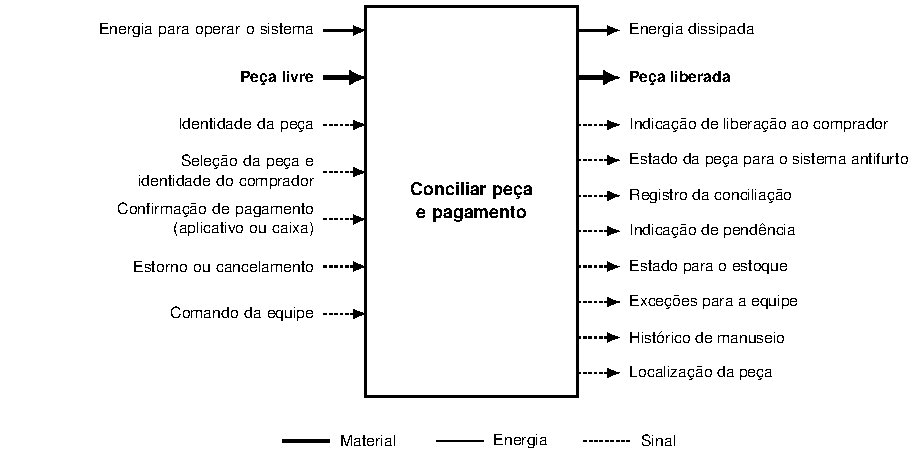
\includegraphics[width=\textwidth]{imagens/modelagem_funcional/modelagem_funcao_total.pdf}
    \label{fig:funcao_total}
    \source{Elaborado pelos autores (2026).}
\end{figure}

A equipe descartou três formulações durante essa definição. \emph{Transferir a posse da peça} trazia a conotação jurídica do termo posse. \emph{Gerenciar a identidade, a proteção e a transferência de posse de uma peça de vestuário} enumerava funções parciais em vez de resumi-las. E formulações centradas na saída da loja, como \emph{controlar a saída da peça}, descreviam uma função que o antifurto existente já cumpre.

A equipe comparou duas posições para o início do sistema: a decisão de compra, com a peça já retida, ou o início da retenção, com a peça livre. Adotou a segunda, para que a função total abrangesse identificar, reter e liberar a peça. Com essa escolha, a peça é o único material que cruza a fronteira, e o elemento que a retém pertence ao sistema, sem figurar como entrada.

A energia de entrada ficou sem forma definida, porque sua natureza depende de princípios de solução ainda não escolhidos; o exemplo de lavagem de roupas apresentado por \citeonline{rozenfeld2006gestao} dá à energia o mesmo tratamento. A saída de energia corresponde à parcela dissipada. A equipe tratou os sinais como informação, sem referência ao meio de transmissão. A confirmação de pagamento pode vir do aplicativo ou do caixa, porque uma peça paga no caixa também precisa ser conciliada. O estorno ou cancelamento antes da saída e o comando da equipe cobrem três situações de exceção: pagamento negado, desistência depois do pagamento e falha do sistema.

A equipe tomou duas decisões levando em conta o que a loja já tem. A primeira é que o sistema não emite alarme, função que permanece com o antifurto já instalado na saída da loja; em contrapartida, precisa informar a esse antifurto o estado da peça conciliada, para que o alarme não dispare para quem pagou. A segunda é que a tentativa de remoção indevida ficou fora dos fluxos de entrada: a equipe a converteu em exigência sobre a manutenção da retenção, a ser quantificada nas especificações e examinada na análise de modos de falha.

\subsection{Estrutura de funções}
\label{sec:estrutura_funcoes}

A equipe representou o desdobramento como estrutura de funções, que mostra os fluxos entre funções. As árvores de funções, segundo \citeonline{rozenfeld2006gestao}, não representam essas interações, e a conciliação depende delas. O desdobramento começou pelos processos que convertem os fluxos principais. O fluxo de material exigiu \emph{reter a peça} (F1) e \emph{liberar a peça} (F3); o fluxo de sinal exigiu \emph{vincular a peça ao pagamento} (F2), cuja saída controla F3. A Figura~\ref{fig:estrutura_funcoes} apresenta a estrutura resultante.

Em F1, a retenção começa sobre a peça livre (F1.1) e se mantém enquanto não houver autorização válida (F1.3). Resistir à remoção indevida e preservar a integridade da peça ficaram registrados como exigências de F1.3, sem formar funções próprias. F1.2 associa a retenção à identidade que a peça já traz, e F3.1 recebe essa associação para identificar qual retenção encerrar. A função F1.2 surgiu da escolha da fronteira, porque a peça entra no sistema sem vínculo com a retenção.

Em F2, o sistema recebe a seleção da peça e a identidade do comprador (F2.1) e a confirmação de pagamento (F2.2), compara a peça com a transação (F2.3) e registra o vínculo (F2.4). F2.5 desfaz o vínculo quando há estorno ou cancelamento antes da saída, e a comparação volta a indicar peça não conciliada.

Em F3, a autorização de liberação chega de F2.3 ou do comando da equipe (F3.1) e aciona três funções: encerrar a retenção (F3.2), indicar a liberação ao comprador (F3.3) e informar o estado da peça ao antifurto existente (F3.4). F3.4 permanece condicional: só será necessária se esse antifurto continuar a detectar a peça depois da liberação, ponto ainda a confirmar com a Riachuelo. A equipe já havia decidido indicar a liberação por sinal luminoso; registrou essa decisão como restrição para a busca de princípios de solução e manteve no modelo apenas a função F3.3. A função auxiliar F0 supre energia às funções que iniciam e encerram a retenção.

A equipe verificou a compatibilidade entre funções adjacentes, exigida pelo método: a peça retida que sai de F1.3 é a entrada material de F3.2, e o vínculo confirmado que sai de F2.3 é a entrada de sinal de F3.1.

\begin{landscape}
\begin{figure}[p]
    \centering
    \caption{Estrutura de funções do sistema, com a classificação das funções em básicas, secundárias necessárias e acessórias}
    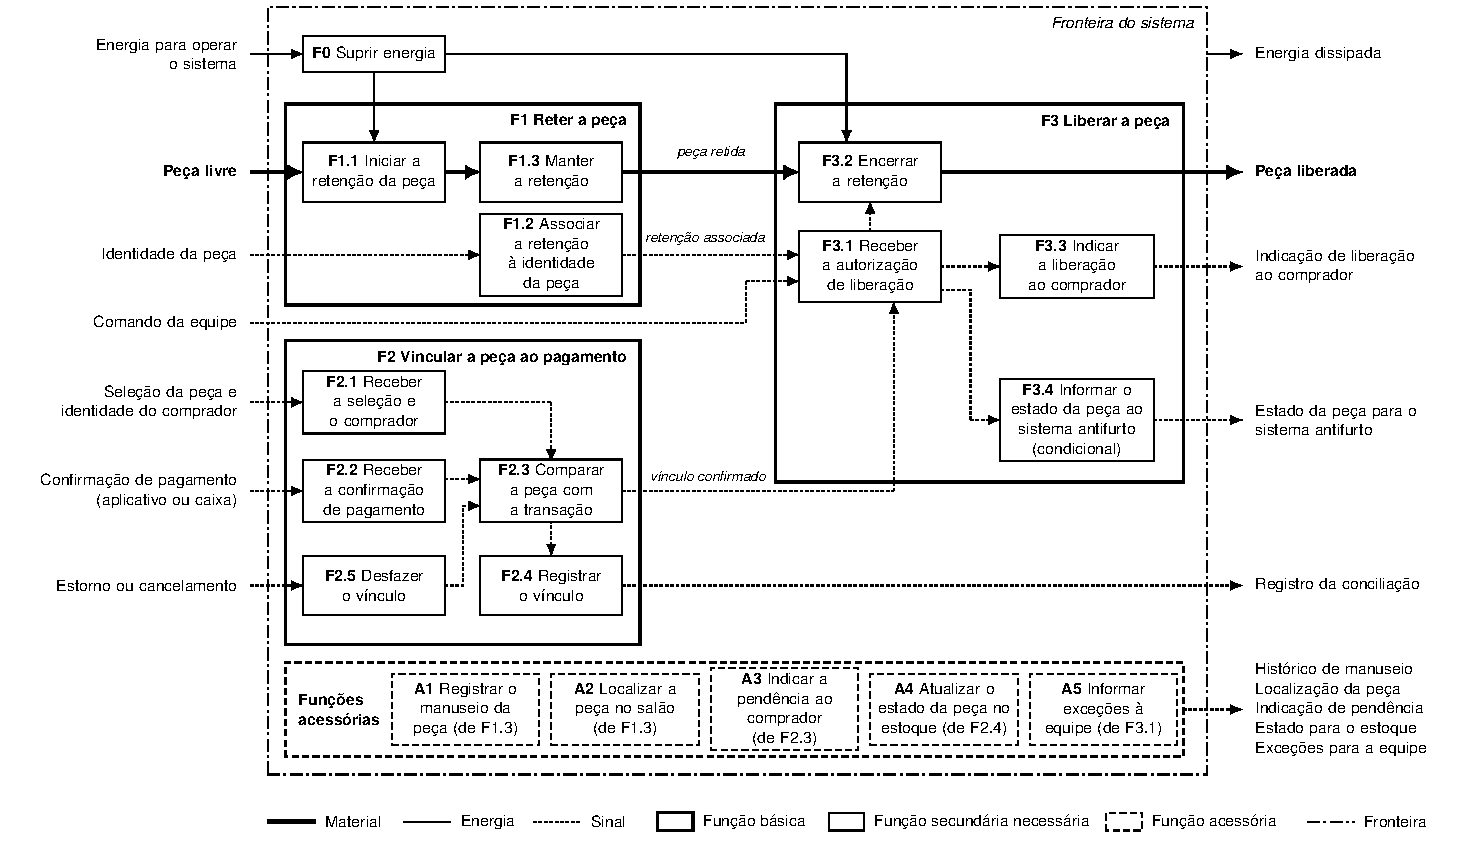
\includegraphics[width=\linewidth]{imagens/modelagem_funcional/modelagem_estrutura_funcoes.pdf}
    \label{fig:estrutura_funcoes}
    \source{Elaborado pelos autores (2026).}
\end{figure}
\end{landscape}

\subsection{Classificação das funções}
\label{sec:classificacao_funcoes}

Para orientar as etapas seguintes, a equipe classificou as funções segundo as categorias da Análise do Valor, método que \citeonline{rozenfeld2006gestao} listam entre os métodos sistemáticos de criatividade sem detalhar essa tipologia. Funções básicas justificam a existência do produto; secundárias necessárias viabilizam as básicas; acessórias agregam valor sem condicionar a conversão dos fluxos principais; funções de estima dizem respeito à percepção de quem usa o produto. Na Figura~\ref{fig:estrutura_funcoes}, F1, F2 e F3 são básicas, e F0 e as funções de segundo nível são secundárias necessárias.

As cinco funções acessórias aproveitam estados já produzidos na estrutura. \emph{Registrar o manuseio da peça} (A1) e \emph{localizar a peça no salão} (A2) partem da peça retida em F1.3; \emph{indicar a pendência ao comprador} (A3) parte de uma comparação sem vínculo em F2.3; \emph{atualizar o estado da peça no estoque} (A4) parte do registro em F2.4; e \emph{informar exceções à equipe} (A5) parte das liberações por comando em F3.1. A conciliação ocorre sem elas. A1, A2 e A4, porém, sustentam a parte da proposta de valor apoiada em dados de interação e de disponibilidade em loja, incluída no escopo do problema.

As funções de estima não aparecem na estrutura, que representa apenas fluxos de energia, material e sinal. A equipe identificou quatro. \emph{Evitar o constrangimento do comprador na saída} e \emph{legitimar a compra perante terceiros} respondem à baixa adesão ao item do survey sobre saída sem checagem manual, que 76\% dos respondentes não endossaram (Figura~\ref{fig:confianca_geral}). \emph{Transmitir autonomia ao comprador} liga-se à dimensão de autonomia discutida na Seção~\ref{sec:clusters}. \emph{Preservar a aparência da peça durante a prova} decorre de a loja ter a peça no corpo do cliente no momento da decisão. Essas funções entraram como critérios na seleção da concepção (Seção~\ref{subsec:reform_escolha}), etapa em que \citeonline{rozenfeld2006gestao} admitem critérios estéticos ao lado das especificações-meta.

A estrutura reúne três funções básicas, treze secundárias necessárias e cinco acessórias. Como o procedimento da matriz morfológica recomenda trabalhar com até dez funções \cite{rozenfeld2006gestao}, a equipe priorizou sete funções na montagem da matriz (Seção~\ref{subsec:reform_matriz}).